\documentclass{anstrans}
\usepackage[utf8]{inputenc}
\usepackage{tikz}
\usepackage{amsmath}
\usetikzlibrary{shapes.misc, shapes.geometric, arrows, positioning}
\tikzstyle{b} = [rectangle, draw, fill=blue!20]
\tikzstyle{c} = [rectangle, draw, fill=red!20]
\tikzstyle{l} = [draw, -latex', thick]
\usepackage{multirow}

\title{Used Nuclear Fuel Inventory Resolution Sensitivity Analysis with UNF-STANDARDS}
\author{Jin Whan Bae$^{1}$, Joshua L. Peterson-Droogh$^{2}$, Kathryn D. Huff$^{1}$}
\institute{
$^{1}$ Dept. of Nuclear, Plasma, and Radiological Engineering, University of Illinois at Urbana-Champaign, Urbana, IL
\and
$^{2}$ Oak Ridge National Laboratory, Oak Ridge, TN}
\date{}

\usepackage[acronym, toc]{glossaries}
\newacronym{NNL}{NNL}{National Nuclear Laboratory}
\newacronym{MA}{MA}{minor actinide}
\newacronym{DU}{DU}{depleted uranium}
\newacronym{LWR}{LWR}{Light Water Reactor}
\newacronym{MOX}{MOX}{Mixed Oxide Fuel}
\newacronym{FBR}{FBR}{Fast Breeder Reactor}
\newacronym{SFR}{SFR}{Sodium-cooled Fast Reactor}
\newacronym{FLM}{FLM}{Fuel Loading Model}
\newacronym{EFMC}{EFMC}{effective fissile mass coefficient}
\newacronym{ORNL}{ORNL}{Oak Ridge National Laboratory}
\newacronym{PWR}{PWR}{Pressurized Water Reactor}
\newacronym{FIT}{FIT}{Functionality Isolation Test}
\newacronym{MSR}{MSR}{Molten Salt Reactor}
\newacronym{PRISM}{PRISM}{Power Reactor Innovative Small Module}
\newacronym{UNF}{UNF}{Used Nuclear Fuel}
\newacronym{EPF}{EPF}{Equivalent Pu-239 Factor}
\newacronym{UNF-STANDARDS}{UNF-ST\&DARDS}{\gls{UNF} Storage, Transportation \& Disposal Analysis Resource and Data System}
\newacronym{PyNE}{PyNE}{Python for Nuclear Engineering}
\begin{document}
\section{Abstract}
Fuel cycle simulations frequently fail to capture the isotopic variation in spent nuclear 
fuel among reactors of the same type. In this paper, we evaluate the validity and limits of 
this simplification by comparing the high-resolution \gls{UNF} inventory in 2020 from the \gls{UNF-STANDARDS} \cite{peterson_used_2013} with a \gls{UNF} inventory generated by 
assuming an average burnup and enrichment.
We additionally compared fuel cycle analysis and waste management metrics calculated using 
each dataset. We found that assuming an averaged inventory negligibly impacts fuel cycle 
analysis metrics, but yields significant error in waste management metrics. However, this 
error decreases to almost zero as the fission products decay over time. We conclude that 
using an average burnup and enrichment to model discharged fuel in the U.S. can be an 
acceptable approximation for fuel cycle analysis.

\section{Introduction}
Fuel cycle simulators often model spent nuclear fuel composition across a fleet of 
reactors with representative compositions or \emph{recipes} \cite{huff_fundamental_2016, jacobson_vision_2010, gregg_analysis_2012, feng_standardized_2016}. This recipe assumption fails 
to capture the true isotopic variation in spent nuclear fuel among reactors of the same type. 
This work explores the potential impact of this assumption on the calculation of metrics 
typically calculated by such simulation tools.

\gls{UNF-STANDARDS} has been developed to integrate
a centralized \gls{UNF} database \cite{peterson_used_2013} and the SCALE suite of codes \cite{noauthor_scale_nodate} to
perform neutronics and thermal hydraulics analysis for 
\gls{UNF} management and disposal analysis.
This comprehensive, high-resolution database lists every \gls{UNF} assembly discharged 
in the U.S ($\sim244,896$) and their properties
(initial enrichment, burnup, ORIGEN-depleted isotopic composition, assembly type, etc.).
While high resolution of this kind is exceptionally valuable, the volume of data can 
present challenges for processing and simulation computation times.

We compare the predicted U.S. \gls{UNF} inventory in 2020 calculated using
\gls{UNF-STANDARDS} to the same prediction calculated using a simplified \gls{UNF} 
inventory assuming an average burnup and enrichment in order to assess the impact of this common simplifying assumption on fuel cycle metric accuracy.

\section{Background}
\gls{UNF} is typically either destined for disposal (after storage) or reprocessing.
Accordingly, the U.S. \gls{UNF} inventory can be analyzed in two different
ways, with certain metrics important for each (listed in Table \ref{tab:met}).

\begin{table}[h]
    \centering
    \begin{tabular}{ccc}
        \hline
        Analysis type & Important metric & Unit\\
        \hline
        Fuel cycle analysis & Equivalent Pu-239 & t \\
        \hline
        \multirow{2}{*}{Waste management} & \shortstack{Decay heat \\ (@ 2020, 2100, 3100)} & MW\\
        & \shortstack{Activity \\ (@ 2020, 2100, 3100)} & Bq \\
        \hline
    \end{tabular}
    \caption{Important metrics for \gls{UNF} with regard to analysis types }
    \label{tab:met}
\end{table}

When considering reprocessing, the most important
factor to consider is the fissile inventory of the \gls{UNF}.
In order to measure the fissile material value of \gls{UNF}, we calculate
the equivalent $^{239}Pu$ value using the table from \cite{anon_plutonium_1989}, reproduced below in Table \ref{tab:pu_equiv}.
The motivation for considering both the \gls{LWR} and the \gls{FBR} case is to
consider different transition scenarios. For example, the LWR factors
would represent recycling the plutonium to create \gls{MOX} for \glspl{LWR} while the \gls{FBR} factors represent using the fissile
materials for a fast reactor, such as a \gls{SFR} or a \gls{MSR}.

\begin{table}[h]
    \centering
    \begin{tabular}{crr}
        \hline
        Isotope & LWR & \shortstack{FBR\\ (Super-Phenix)} \\
        \hline
        $^{235}U$ & +0.8 & +0.800 \\
        $^{238}Pu$ & -1.0 & +0.440 \\
        $^{239}Pu$ & +1.0 & +1.000 \\
        $^{240}Pu$ & -0.4 & +0.140 \\
        $^{241}Pu$ & +1.3 & +1.500 \\
        $^{242}Pu$ & -1.4 & +0.037 \\
        $^{241}Am$ & -2.2 & -0.330 \\
        \hline
    \end{tabular}
    \caption{Equivalent $^{239}Pu$ factors for each isotope in thermal (LWR) and fast (FBR) spectra,
             reproduced from \cite{anon_plutonium_1989}.}
    \label{tab:pu_equiv}
\end{table}

Using the table, the total `equivalent $^{239}Pu$' for a material is
calculated with this formula:

\[ Pu_{eq} = \sum{F_i \cdot M_i} \]
\[ F_i = \text{Equivalence factor for isotope i}\]
\[ M_i = \text{Mass of isotope i} \]

In \gls{UNF} management analysis, important metrics include
decay heat and activity. Since these
change over time, we calculate and compare the metrics
at various times: the near present (2020), near future (2100), and far future (3100).
Table \ref{tab:met} lists the metrics used to compare the 
two \gls{UNF} inventory datasets.

\section{Methodology}
We used the nuclear engineering data toolkit, \gls{PyNE} \cite{scopatz_pyne_2012},
to analyze the impact of simplifying spent fuel compositions in fuel cycle 
metrics calculations. First, 
we validated the decay function in \gls{PyNE} against \gls{UNF-STANDARDS}, 
which uses ORIGEN \cite{bell_origen:_1973} to perform decay calculations.

We then used \gls{PyNE} to simulate the decay of
discharged \gls{UNF} to 2020, and compared resulting cumulative composition 
with the results from \gls{UNF-STANDARDS}.

Next, we found the average
burnup and enrichment in the \gls{UNF} database to establish 
the composition of the average fuel assembly.
We stored this composition and assume that all fuel
discharged is depleted to this composition. Finally, we
compared the total \gls{UNF} inventory and 2020 composition 
isotopics in the simplified case (assuming one spent fuel 
composition) with the high-resolution case (many assembly-specific 
compositions in the \gls{UDB}).

\subsection{PyNE and ORIGEN decay comparison}
To ensure the validity of the decay function implemented in \gls{PyNE}, 
we imported the database into \gls{PyNE} and decayed each assembly
to 2020. A comparison of the resulting \gls{PyNE} inventory with the 2020 inventory generated by \gls{UNF-STANDARDS} appears in Table \ref{tab:avg}. 
The table shows that the \gls{PyNE} results have excellent
agreement with the ORIGEN results via \gls{UNF-STANDARDS}.

\begin{table}[h]
    \centering
    \begin{tabular}{lrrr}
        \hline
        Metric & PyNE & ORIGEN & $\Delta$ \\
        \hline
        $^{239}Pu$ mass [t] & 520.52 & 520.50 & 0.02\\
        $^{137}Cs$ mass [t] & 59.23 & 59.19 & 0.04\\
        $^{235}U$ mass [t] & 771.42 & 771.39 & 0.03\\
        Total mass [t] & 68,072 & 67,984 & 88\\
        Decay Heat [MW] & 61.31 & 61.10 & 0.21 \\
        Activity [Bq] & $6.76e20$ & $6.74e20$ & 0.02e20 \\
        \hline
    \end{tabular}
    \caption{Comparison between \gls{PyNE} decayed and ORIGEN decayed \gls{UNF} inventory in 2020.}
\end{table}

\subsection{Average Assembly}
We established an average assembly composition by first finding the
average burnup and enrichment values in the database,
and then finding an assembly that has the closest
burnup and enrichment values to the average.
The average burnup of the assemblies in the \gls{UDB} was $36.169 MWD/MTHM$
and the average enrichment was $3.39 \% ^{235}U$. With these
average values, we selected an assembly closest to the
average. Table \ref{tab:avg} lists the composition of the selected assembly.

\begin{table}[h]
    \centering
    \begin{tabular}{cr}
        \hline
        Isotope & wt \% \\
        \hline
        $^{238}U$ & 96.5000 \\
        $^{235}U$ & 1.0400 \\
        $^{241}Am$ & 0.0160 \\
        $^{239}Pu$ & 0.7550   \\
        $^{137}Cs$ & 0.1320   \\
        ${90}Sr$ & 0.0552  \\
        Pu Total & 1.2760   \\
        \hline
    \end{tabular}
    \caption{Composition of the representative
             assembly selected for analysis.}
    \label{tab:avg}
\end{table}

\section{Results}
The results show that the simplified case yields a small
error for the fuel cycle analysis metrics, and a time-varying
error for the waste management metrics.

\subsection{Simplified Inventory and High-resolution Inventory Comparison.}
We calculated the isotopic differences between the two cases
and the metrics important for both fuel cycle analysis
and waste management.

The mass difference and relative difference values are calculated
with the following formula:
\[\Delta M_i = M_{HR} - M_{S} \]
\[\text{Rel. Error} = \frac{M_{HR} - M_{s}}{M_{HR}}\]
\[M_{HR} = \text{Isotope mass in inventory (high-resolution case)}\]
\[M_{S} = \text{Isotope mass in inventory (simplified case)}\]

The absolute and relative mass differences
of important isotopes between two cases are shown in
Figures \ref{fig:iso_mass} and \ref{fig:iso_rel}. 
The figures show that the simplified case yields
large errors for fission products and $^{241}Am$, $^{244}Cm$, and $^{235}U$,
which depend significantly on burnup and initial enrichment.
Meanwhile, the 80-ton mass difference in $^{238}U$ does not
translate into a substantial relative error due to its massive
total inventory.

\begin{figure}
    \centering
    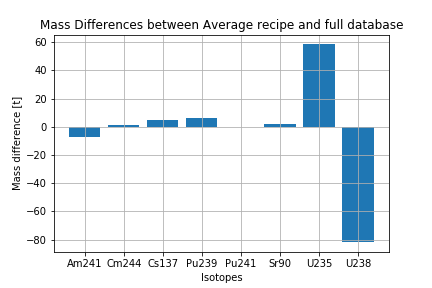
\includegraphics[width=0.45\textwidth]{iso_mass.png}
    \caption{Mass difference between high resolution and simplified case for different isotopes.}
    \label{fig:iso_mass}
\end{figure}

\begin{figure}
    \centering
    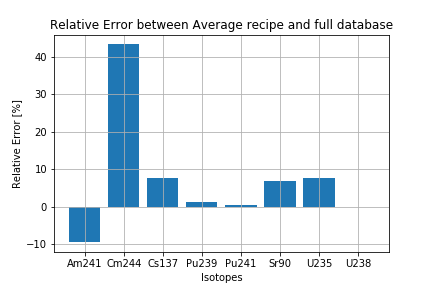
\includegraphics[width=0.45\textwidth]{iso_rel.png}
    \caption{Relative error between high resolution and simplified case for different isotopes.}
    \label{fig:iso_rel}
\end{figure}

The same plots are generated for different plutonium
isotopes in Figures \ref{fig:pu_mass} and \ref{fig:pu_rel}.
The figures show that the simplified case under-calculates
all plutonium isotopes except for $^{240}Pu$, and that the
simplified case has 10 tons less plutonium than the
high-resolution case.

\begin{figure}
    \centering
    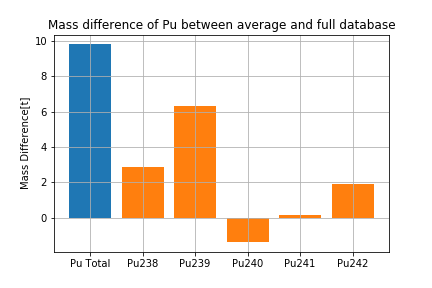
\includegraphics[width=0.45\textwidth]{pu_mass.png}
    \caption{Mass difference between high resolution and simplified case for plutonium isotopes.}
    \label{fig:pu_mass}
\end{figure}

\begin{figure}
    \centering
    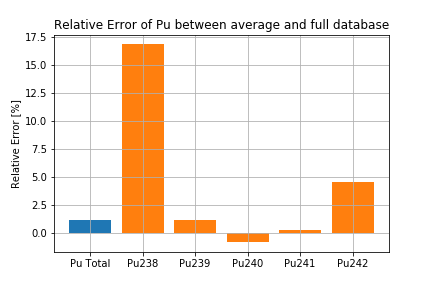
\includegraphics[width=0.45\textwidth]{pu_rel.png}
    \caption{Relative error between high resolution and simplified case for plutonium isotopes.}
    \label{fig:pu_rel}
\end{figure}

\subsubsection{Waste Management Metrics}
The two major waste management metrics are radioactivity and
decay heat. Since the two metrics change in time, the metrics
are evaluated in three different times, in 2020, 2100 (short future),
and 3100 (far future). The results are shown in Table \ref{tab:wm} and
Figures \ref{fig:heat}, \ref{fig:act}, and \ref{fig:wm_err}.

\begin{table}[h]
    \centering
    \begin{tabular}{lcrrr}
        \hline
        Metric & Year & HR case & Simpl. Case  & Rel. Err. [\%]\\
        \hline
        \multirow{3}{*}{\shortstack{Decay \\ Heat}} & 2020 & 61.31 & 53.90 & 12.08 \\
                                                    & 2100 & 24.27 & 23.63 & 2.63\\
                                                    & 3100 & 4.72 & 4.83 & -2.45\\
        \hline
        \multirow{3}{*}{\shortstack{Activity}} & 2020 & 6.76e20 & 6.33e20 & 6.27\\
                                               & 2100 & 9.28e19 & 8.76e19 & 5.59\\
                                               & 3100 & 5.54e18 & 5.654e18 & -2.02\\
        \hline
    \end{tabular}
    \caption{Decay heat and radioactivity values and errors for years 2020, 2100, and 3100.}
    \label{tab:wm}
\end{table}


These results demonstrate that the error decreases with time, meaning that the error 
stems from the inaccuracy of the simplified case to take into account the short-lived 
fission products (e.g. $^{137}Cs$, $^{90}Sr$), as shown in Figure \ref{fig:iso_rel}. The
error becomes negative after 2200, likely because the simplified
case contains 10\% more $^{241}Am$ in its inventory.

\begin{figure}
    \centering
    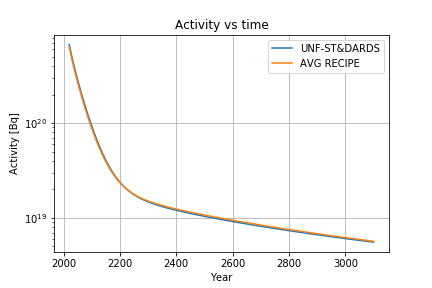
\includegraphics[width=0.45\textwidth]{activity.png}
    \caption{Activity of the \gls{UNF} inventory for simplified and
            high resolution case.}
    \label{fig:act}
\end{figure}

\begin{figure}
    \centering
    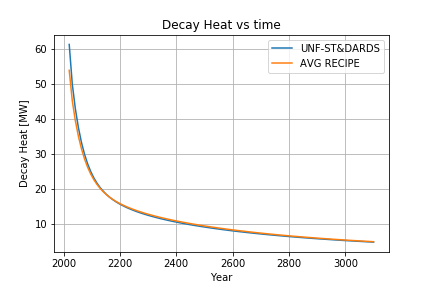
\includegraphics[width=0.45\textwidth]{heat.png}
    \caption{Decay heat of the \gls{UNF} inventory for simplified
             and high resolution  case.}
    \label{fig:heat}
\end{figure}

\begin{figure}
    \centering
    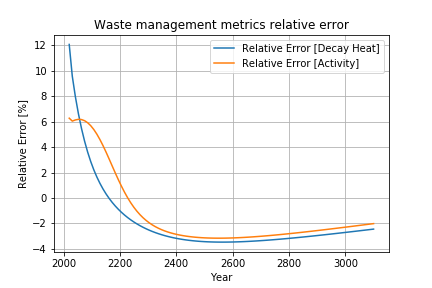
\includegraphics[width=0.45\textwidth]{ha_err.png}
    \caption{Relative error of activity and decay heat of the
            \gls{UNF} inventory over time.}
    \label{fig:wm_err}
\end{figure}

In the future, the \gls{UNF} inventory can be reprocessed
for its plutonium and uranium, leaving the remainder (fisison
products, minor actinides) as high level waste. We separate the 
uranium and plutonium from the \gls{UNF} inventory and calculate 
the \gls{HLW} profile differences for both cases in table
\ref{tab:hlw}.

\begin{table}[h]
    \centering
    \begin{tabular}{cccc}
        \hline
        Category & UDB & Recipe & Rel. Error [\%] \\
        \hline
        \gls{HLW} Mass [t]& 499.4 & 490.8 & 1.7\\
        \gls{HLW} Decay heat [MW] & 49.3 & 43.5 & 11.7 \\
        \gls{HLW} Activity [Bq] & 4.9e20 & 4.5e20 & 8.1\\
        \hline
    \end{tabular}
    \caption{Difference in reprocess waste (\gls{HLW}) for
            high-resolution and simpilified case.}
    \label{tab:hlw}
\end{table}

\subsubsection{Fuel Cycle Analysis Metrics}
Given the isotopic compositions of the \gls{UNF} profile in 2020,
we calculate the equivalent $^{239}Pu$ for both cases, for
both spectra. The results are shown in Table \ref{tab:equiv}.
The figures show that the equivalent
$^{239}Pu$ difference between two cases is 7\% for thermal,
and less than 5\% for fast spectra.

\begin{table}[h]
    \centering
    \begin{tabular}{ccc}
        \hline
        Category & Equiv. $^{239}Pu$ ton & Rel. Error [\%] \\
        \hline
        HR thermal & 880.5 & \multirow{2}{*}{7.28}\\
        Simplified thermal & 816.4\\
        \hline
        HR fast & 1214.0 & \multirow{2}{*}{4.67}\\
        Simplified fast & 1157.3 &\\
        \hline
    \end{tabular}
    \caption{Equivalent $^{239}Pu$ ton value comparison for High-resolution and simplified case.}
    \label{tab:equiv}
\end{table}

To explain this error, we plotted every assembly and its
normalized equivalent $^{239}Pu$, shown in Figures \ref{fig:fast_all} and \ref{fig:thermal_all}.
The normalized equivalent $^{239}Pu$ is simply the 
total equivalent $^{239}Pu$ divided by the total mass
of the assembly.

\begin{figure}
    \centering
    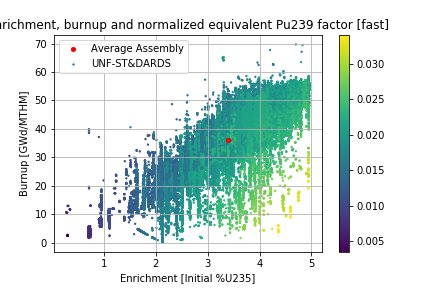
\includegraphics[width=0.45\textwidth]{fast_all.png}
    \caption{All assemblies in the database and their normalized equivalent Pu-239 in a fast reactor.}
    \label{fig:fast_all}
\end{figure}

\begin{figure}
    \centering
    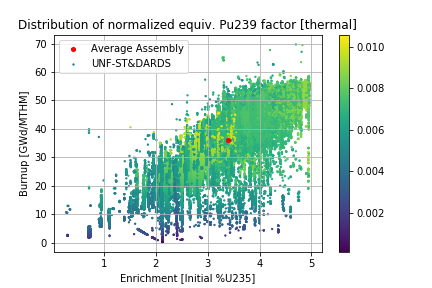
\includegraphics[width=0.45\textwidth]{thermal_all.png}
    \caption{All assemblies in the database and their normalized equivalent Pu-239 in a thermal reactor.}
    \label{fig:thermal_all}
\end{figure}

The scatter plot shows the \gls{UNF}
has a higher normalized equivalent $^{239}Pu$ when the
initial enrichment is high and the burnup high. For the fast spectrum case in \ref{fig:fast_all}, the equivalent $^{239}Pu$ is higher than the thermal spectrum for high burnup, since plutonium isotopes 
build up with higher burnup.

\subsubsection{Transition Scenario differences}
To observe the differences between the high-resolution
and recipe \gls{UNF} inventory in a U.S.
transition scenario to \glspl{SFR}, we perform a parameter sweep on a range
of nuclear energy demand growth rates and \gls{SFR} transition
start years (table \ref{tab:param}). 
There is no difference in the success of transition between
the high-resolution case and the recipe case.

\begin{table}[h]
    \centering
    \begin{tabular}{cc}
        \hline
        Parameters & Values \\
        \hline
        \shortstack[c]{Energy demand\\ growth rate} & 0, 0.5, 1, 1.5 \\
        \lbrack$\%$ per year\rbrack & \\
        \hline
        \shortstack{\gls{SFR} transition \\ start year} & \shortstack{2030, 2035, 2040,\\ 2045, 2050}\\
        \hline
    \end{tabular}
    \caption{Parameters used for transition scenario}
    \label{tab:param}
\end{table}

\begin{table}[h]
    \centering
    \begin{tabular}{cc|cccc}
    \hline
    & & \multicolumn{4}{c}{Energy Demand Growth Rate \lbrack\%\rbrack} \\
    & & 0 & 0.5 & 1.0 & 1.5 \\
    \hline
    & 2030 & - & - & \textcolor{red}{ALL} & \textcolor{red}{ALL} \\
    \multirow{4}{*}{\shortstack{\gls{SFR} \\ \\ Available \\ \\ Year}}& 2035 & - & - & - & \textcolor{red}{ALL} \\
    & 2040 & - & - & - & - \\
    & 2045 & - & - & - & - \\
    & 2050 & - & - & - & - \\
    \hline
    \end{tabular}
    \caption{Transition failure cases. `\textcolor{red}{ALL}' denotes transition failure for both cases.}
    \label{tab:trans_fail}
\end{table}


\section{Conclusion and Discussion}
In this paper, we compared the simplified \gls{UNF}
inventory and the high-resolution \gls{UNF} inventory
at 2020 by calculating the isotopic differences as well
as important metrics for waste management and fuel cycle analysis.
We conclude that the simplified inventory is not adequate for waste
management analysis since the fission products and \glspl{MA}, that are sensitive to 
initial enrichment and burnup, are important when considering
waste management metrics, such as short and long-term decay heat and radioactivity.
Also, in waste management, it is important to consider each assembly separately,
thus having a metric for the entire inventory is inadequate for characterizing the waste inventory.
On the other hand, we found out that the simplified case can be a good
approximation of the \gls{UNF} inventory in terms of fuel cycle analysis,
given that the equivalent $^{239}Pu$ error for fast reactors is less than
5\%. Also, given that most fuel cycle simulators are fleet-based, and
because of the number of depletion calculations involved in a fuel cycle
simulation, high-resolution \gls{UNF} compositions require intensive computation.
The results from this paper support the view that using recipes (pre-determined, representative
discharge compositions) are `good-enough' for preliminary fuel cycle simulations.


\section{Acknowledgements}
The work done was funded through the Nuclear Engineering Science
Laboratory Synthesis (NESLS) program. We thank Kaushik Banerjee
from Oak Ridge National Laboratory for providing the data used
in this paper. 

\bibliographystyle{ans}
\bibliography{bib}


\end{document}
